% --------------------------------------------------------------
% This is all preamble stuff that you don't have to worry about.
% Head down to where it says "Start here"
% --------------------------------------------------------------
 
\documentclass[12pt]{article}
 
\usepackage[margin=1in]{geometry} 
\usepackage{amsmath,amsthm,amssymb,bm}
\usepackage{mathtools}
\usepackage{graphicx}
\usepackage{tikz}
\usepackage{subfig}
 
\newcommand{\N}{\mathbb{N}}
\newcommand{\Z}{\mathbb{Z}}
 
\newenvironment{theorem}[2][Theorem]{\begin{trivlist}
\item[\hskip \labelsep {\bfseries #1}\hskip \labelsep {\bfseries #2.}]}{\end{trivlist}}
\newenvironment{lemma}[2][Lemma]{\begin{trivlist}
\item[\hskip \labelsep {\bfseries #1}\hskip \labelsep {\bfseries #2.}]}{\end{trivlist}}
\newenvironment{exercise}[2][Exercise]{\begin{trivlist}
\item[\hskip \labelsep {\bfseries #1}\hskip \labelsep {\bfseries #2.}]}{\end{trivlist}}
\newenvironment{reflection}[2][Reflection]{\begin{trivlist}
\item[\hskip \labelsep {\bfseries #1}\hskip \labelsep {\bfseries #2.}]}{\end{trivlist}}
\newenvironment{proposition}[2][Proposition]{\begin{trivlist}
\item[\hskip \labelsep {\bfseries #1}\hskip \labelsep {\bfseries #2.}]}{\end{trivlist}}
\newenvironment{corollary}[2][Corollary]{\begin{trivlist}
\item[\hskip \labelsep {\bfseries #1}\hskip \labelsep {\bfseries #2.}]}{\end{trivlist}}
\newenvironment{question}[2][Question]{\begin{trivlist}
\kern10pt
\item[\hskip \labelsep {\bfseries #1}\hskip \labelsep {\bfseries #2.}]}{\end{trivlist}}

% \newcommand*{\answer}{%
%   \par
%   \kern1pt
%   \begingroup
%     \centering
%     \raisebox{.2\baselineskip}{%
%       \textcolor{gray}{
% 	    \rule{.6667\linewidth}{.1pt}%
%       }
%     }%
%     \par
%   \kern8pt
%   \endgroup
% }
\newcommand\TODO[1]{\textcolor{red}{#1}}

\begin{document}
 
% --------------------------------------------------------------
%                         Start here
% --------------------------------------------------------------
 
%\renewcommand{\qedsymbol}{\filledbox}
 
\title{DD2434 Machine Learning, Advanced Course Assignment 1}
\author{Lin Chun Hung, chlin3@kth.se} 
 
\maketitle

% ====================================================================
% Question 1
\begin{question}{1}
% TODO: Fix the arguments
Consider input output pairs are linked by the mapping to have the following
 relation:
\begin{equation}
    \textbf{t}_i = f(\textbf{x}_i) + \bm{\epsilon}
\end{equation}
where the $\bm{\epsilon}$ is the unbiased random noise. Since we have no piror knowledge
on the random noise term, the random noise is then assumed as following the normal
distribution. \textbf{TODO: More on this}\\

With the assumption that features are uncorrelated, we choose the spherical
covariance matrix for the likelihood.
\end{question} % End question 1
% ====================================================================

% ====================================================================
% Question 2
\begin{question}{2}
Consider the general product rule of probability:
$$\mathrm {P} \left(\bigcap _{k=1}^{n}A_{k}\right)=
  \prod _{k=1}^{n}\mathrm {P} \left(A_{k}\,{\Bigg |}\,\bigcap _{j=1}^{k-1}A_{j}\right)$$

Therefore the likelihood would be:
\begin{equation}
  p(\textbf{T}\mid f,\textbf{X}) =
  \prod _{i=1}^{N}p(\textbf{t}_i \mid \textbf{t}_{i-1},...,\textbf{t}_{1},
  f,\textbf{X})
\end{equation}

\end{question} % End question 2
% ====================================================================

% ====================================================================
% Question 3 
\begin{question}{3}

\begin{equation}
  p(\textbf{T}\mid \textbf{X},\textbf{W}) =
  \prod _{i=1}^{N}N(\textbf{W}\textbf{x}_i, \sigma^2\textbf{I})
\end{equation}
\end{question} % End question 3
% ====================================================================
% ====================================================================
% Question 4
\begin{question}{4}
The choice of piror distribution reflects the choice of regularizer. Chossing L1 
norm as regularizer is known as the lasso (least absolute shrinkage and selection operator).
The regularizer will force some weighting coefficients $w_j$ to be zero, given 
a proper choice of model parameter $\tau$. It plays the role of feature selection
since those zero weighting coefficients indicate that the corresponding features
are irrelvant to the output. \\ 

The penalization term or the negative log-prior:
\begin{equation}
  \frac{\lambda}{2} \left \|vec(W - W_0)\right \|_{q}  % Fix this eqn
\end{equation}

\begin{figure}[h!]
  \centering
  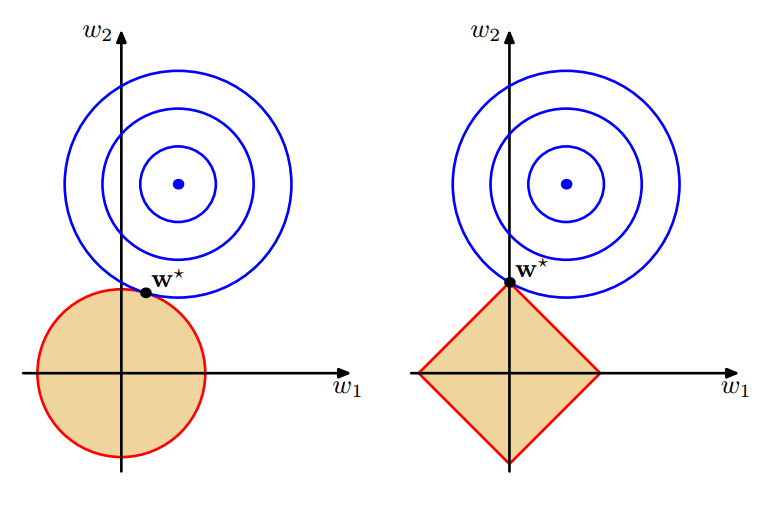
\includegraphics[width=0.5\linewidth]{q4_regular.png}
  \caption{A boat.}
  \label{fig:boat1}
\end{figure}
\end{question} % End question 4
% ====================================================================





% --------------------------------------------------------------
%     You don't have to mess with anything below this line.
% --------------------------------------------------------------
 
\end{document}
